The purpose is to predict the total hourly wind production available on the energy market from all of western Denmark (DK1). It is important to note that it is the wind production available on the market and not the entire production of Western Denmark. This can also be seen by the correlation between consumption and wind production in Table~\ref{table:pearsonCoeficientWindProduction} and Figure~\ref{fig:consumptionVsWindProduction} which indicates that the production is moved into the market when the demand for electricity is high. Because the wind production follows market trends it is necessary to consider economical and statistical factors of the current market situation when predicting the production. It is our intention to get a close enough estimate so that it can be used as an indicator for the hourly amount of wind production in the market for the next 24 hours.
Most others have been forecasting the wind production for specific wind farms where exact weather conditions and wind mill throughput of the site is known beforehand. The assumption is that we loose accuracy without the actual throughputs of the windmills because it is directly proportional to the meteorological factors as presented in~\ref{sec:windmillPlacement}. 

It is not surprising that weather conditions directly impact the wind power generation. The typical input parameters for wind power prediction are wind speed, air density, temperature and pressure \cite{WindPowerGenerationUsingANN} with the most influential factor being wind speed because it is directly converted to power in the wind turbine. The following subsections will describe the parameters relationship to wind production and how it is used in the modelled ANN.

The Pearson Correlation Coefficient\footnote{\url{http://en.wikipedia.org/wiki/Pearson_product-moment_correlation_coefficient}} has been used to establish the linear dependency between meteorological factors, consumption and wind production. Table ~\ref{table:pearsonCoeficientWindProduction} shows this correlation coefficient. The factors have been discussed throughout the thesis as having an influence on the wind speed production to some degree. The Pearson Correlation Coefficient returns a value between -1 and +1 which indicates the strength of the linear correlation between two variables.

\begin{table}[H]
\centering  % used for centering table
\begin{tabular}{c c} % centered columns (3 columns)
Input factor & Pearson Correlation Coefficient \\ [0.5ex] % inserts table 
%heading
\hline                  % inserts single horizontal line
Consumption & 0.61 \\ % inserting body of the table
Wind Speed & 0.94 \\
Temperature & -0.09 \\
Wind Direction & 0.21 \\ [1ex] % [1ex] adds vertical space
\hline %inserts single line
\end{tabular}
\caption{Table showing Pearson correlation coefficient between various factors and the wind production.} % title of Table
\label{table:pearsonCoeficientWindProduction} % is used to refer this table in the text
\end{table}

Table~\ref{table:pearsonCoeficientWindProduction} shows that consumption and wind speed are the most direct influential factors.

\subsection{Meteorological factors}

\subsubsection{Wind Speed}
Wind speed is directly proportional to wind production as described in Section~\ref{sec:windmillPlacement} \todo{discuss reliability of the formula}. This relationship between hourly wind speed and hourly wind power production of DK1 is seen in Figure~\ref{fig:windVsProd}. The graph clearly shows the expected impact of wind speed on the wind energy production. The established Pearson co-relation between wind production and wind speed is further seen in Figure~\ref{fig:windSpeedWindProductionPlot} where the wind production follows the same trend as wind speed for the beginning of 2012. The hours are representative for the whole year \todo{ref to appendix} which is also backed up by the good co-relation. 

\begin{figure}[H]
\centering
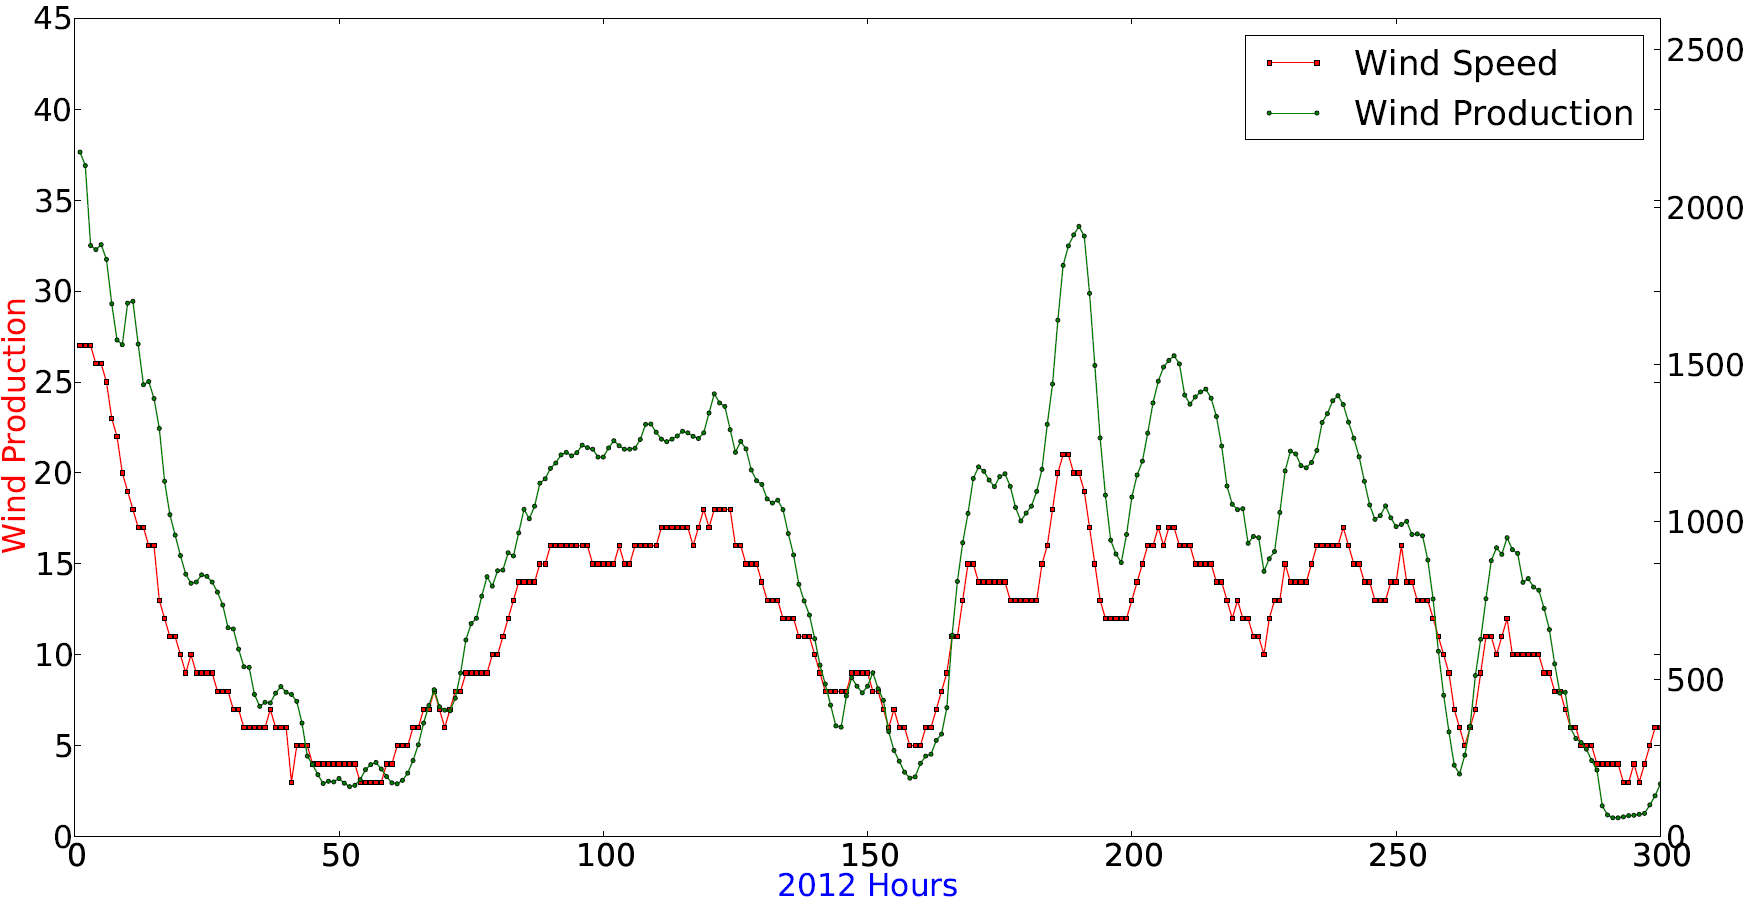
\includegraphics[width=0.99\linewidth,natwidth=898,natheight=587]{billeder/windSpeedWindProductionPlot.png}
\caption{Wind speed and wind production in diagram}
\label{fig:windSpeedWindProductionPlot}
\end{figure}

\begin{figure}[H]
\centering
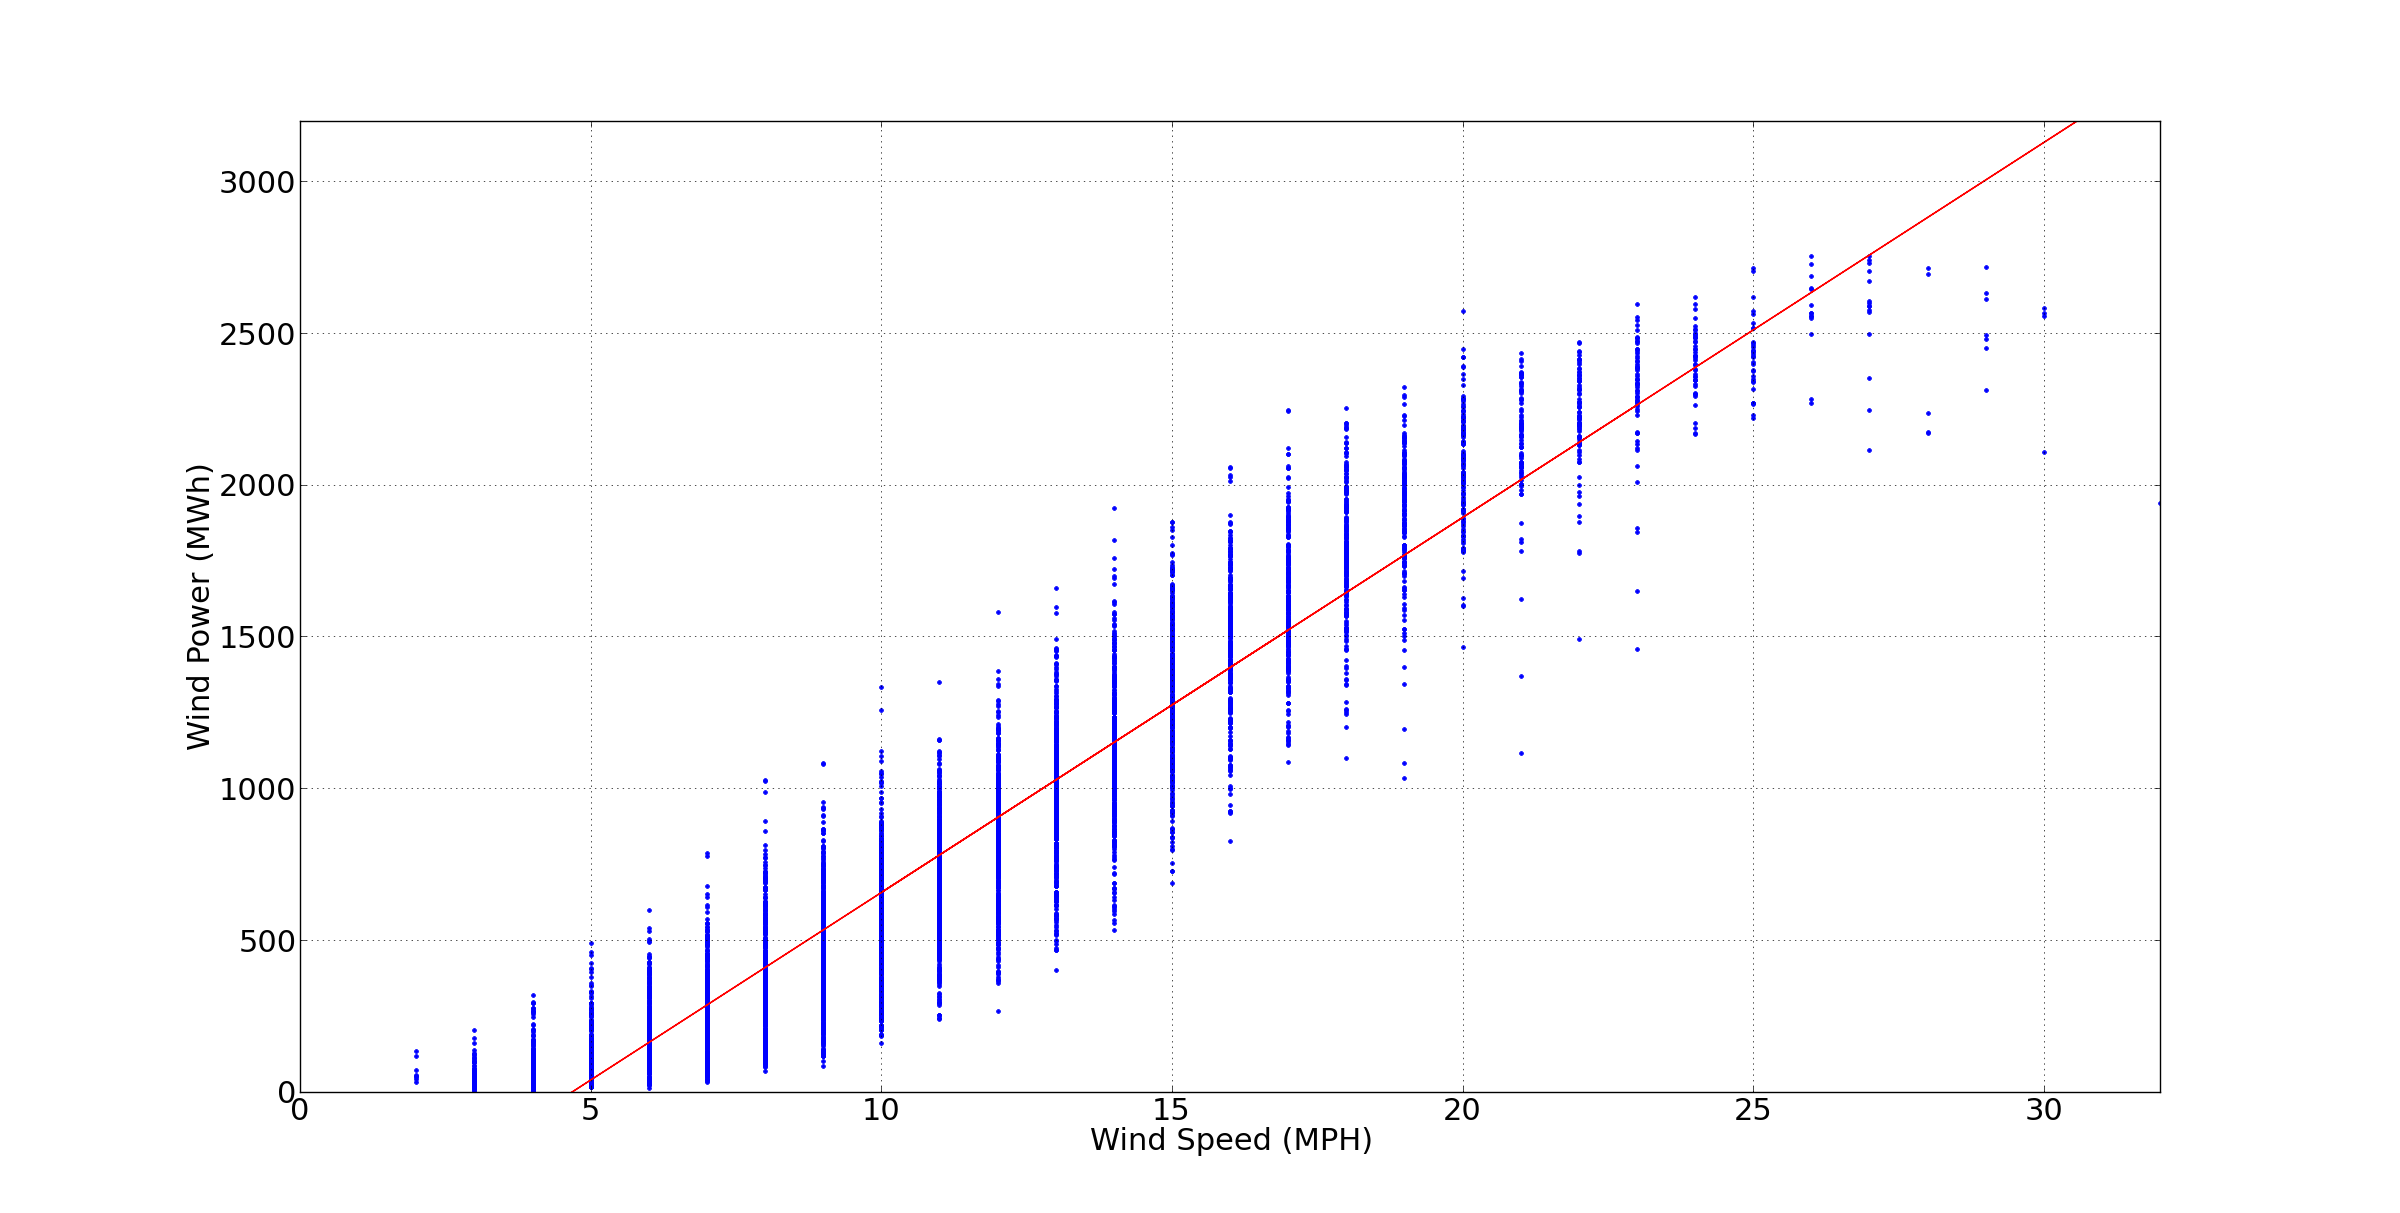
\includegraphics[width=0.99\linewidth,natwidth=898,natheight=587]{billeder/WindSpeedVsProduction.png}
\caption{Wind speed vs. wind production in beginning 2012}
\label{fig:windVsProd}
\end{figure}

What is noticeable from the graphs is wide range of productions that is covered by a relatively small number of wind speeds. Wind speed 15 can cover wind productions all the way from 700 to 1900 and therefore other input parameters are needed to point us in the right direction within these interval. 

\subsubsection{Air Density}
\label{sec:airDensity}
It is described in Section~\ref{sec:windmillPlacement} that wind energy is proportional to air density where a higher density means more power for a specific wind speed. This does not imply that a higher air density is equal to higher wind power production in general because it depends on the wind speed. Days with equal wind speed but variation in air density should show an increase in power production when the air density is highest. 

Air density depends directly on temperature and pressure which can be described by $Air Density=\frac{P*M}{(R*T)}$ where R is a gas constant and M is the mass of dry air. The monthly pressure in Denmark has low variation compared to the temperature as shown in Figure~\ref{fig:pressureTemperatureVariance}. For this reason, the temperature will have the most influence on the air density in Denmark and it might even be enough to leave out pressure and only include temperature. The formula express that when temperature decreases the air density will increase linearly, e.g. the wind power production for a specific wind speed will be higher in times of low temperature. The air density has been calculated for every hour in the training set and the correlation has been established for each wind speed in Table~\ref{table:pearsonCoeficientAirDensity}. The wind power production increases with the air density for each wind speed as described by the formula.

\begin{figure}[H]
\centering
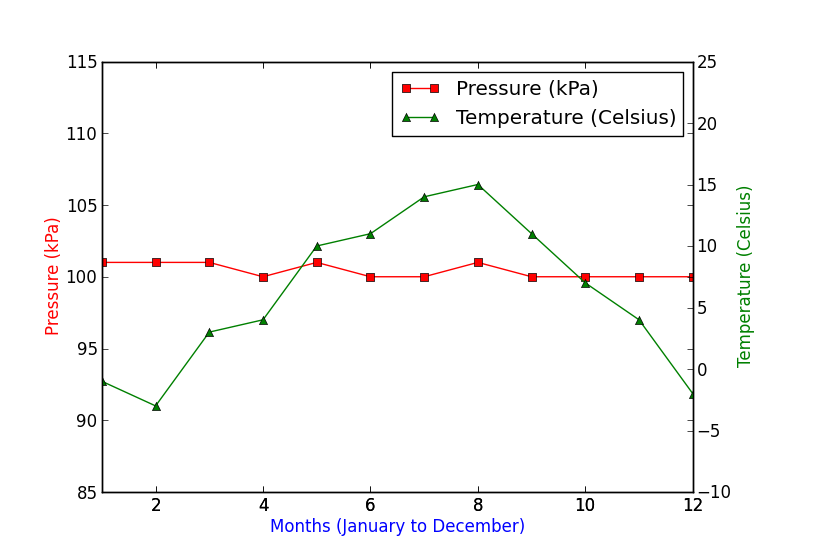
\includegraphics[width=0.99\linewidth,natwidth=898,natheight=587]{billeder/pressureTemperatureVariance.png}
\caption{Temperature and Pressure variance for 2012}
\label{fig:pressureTemperatureVariance}
\end{figure}

\begin{table}[H]
\centering  % used for centering table
\begin{tabular}{c c} % centered columns (3 columns)
Wind Speed (mph) & Pearson Correlation Coefficient for Air Density \\ [0.5ex] % inserts table 
%heading
\hline                  % inserts single horizontal line
2 & 0,29\\ \hline
3 & 0,38 \\ \hline
4 & 0,28 \\ \hline
5 & 0,18 \\ \hline
6 & 0,27 \\ \hline
7 & 0,26 \\ \hline
8 & 0,29 \\ \hline
9 & 0,31 \\ \hline
10 & 0,28  \\ \hline
11 & 0,18 \\ \hline
12 & 0,19 \\ \hline
13 & 0,19 \\ \hline
14 & 0,19 \\ \hline
15 & 0,12 \\ \hline
16 & 0,10 \\ \hline
17 & 0,22 \\ \hline
18 & 0,11 \\ \hline
19 & 0,28 \\ \hline
20 & 0,11 \\ \hline
21 & 0,18 \\ \hline
22 & 0,18 \\ \hline
23 & 0,26 \\ \hline
24 & 0,01 \\ \hline
25 & 0,12 \\ \hline
26 & 0,20 \\ \hline
27 & 0,72 \\ \hline
28 & 0,87 \\ \hline
29 & 0,61 \\ \hline
30 & 0,76 \\ \hline  
Average: & 0,28 \\ [1ex] % [1ex] adds vertical space      
\hline %inserts single line
\end{tabular}
\caption{Table showing Pearson correlation coefficient between the various wind speeds in the dataset and the air density.} % title of Table
\label{table:pearsonCoeficientAirDensity} % is used to refer this table in the text
\end{table}

\subsubsection{Wind Direction}
Figure~\ref{fig:windDirVsProd} shows that the wind direction in general has an impact on the wind production which can also be seen in the co-relation constant from Table~\ref{table:pearsonCoeficientWindProduction}. The wind direction is expected to have a small influence based on Section~\ref{sec:windmillPlacement} where it is described how change in wind direction affect placement of windmills. The wind speed could be more powerful when coming from a specific direction which differs according to the physical location. It needs to be validated in experiments if the wind direction makes sense in relation to the other parameters used as input.
 
\begin{table}[H]
\centering  % used for centering table
\begin{tabular}{c c} % centered columns (3 columns)
Input factor & Pearson Correlation Coefficient \\ [0.5ex] % inserts table 
%heading
\hline                  % inserts single horizontal line
Wind Production & 0.21 \\ % inserting body of the table
Wind Speed & 0.20 \\ [1ex] % [1ex] adds vertical space
\hline %inserts single line
\end{tabular}
\caption{Table showing Pearson correlation coefficient between various factors and the wind direction.} % title of Table
\label{table:pearsonCoeficientWindDirection} % is used to refer this table in the text
\end{table}

\begin{figure}[H]
\centering
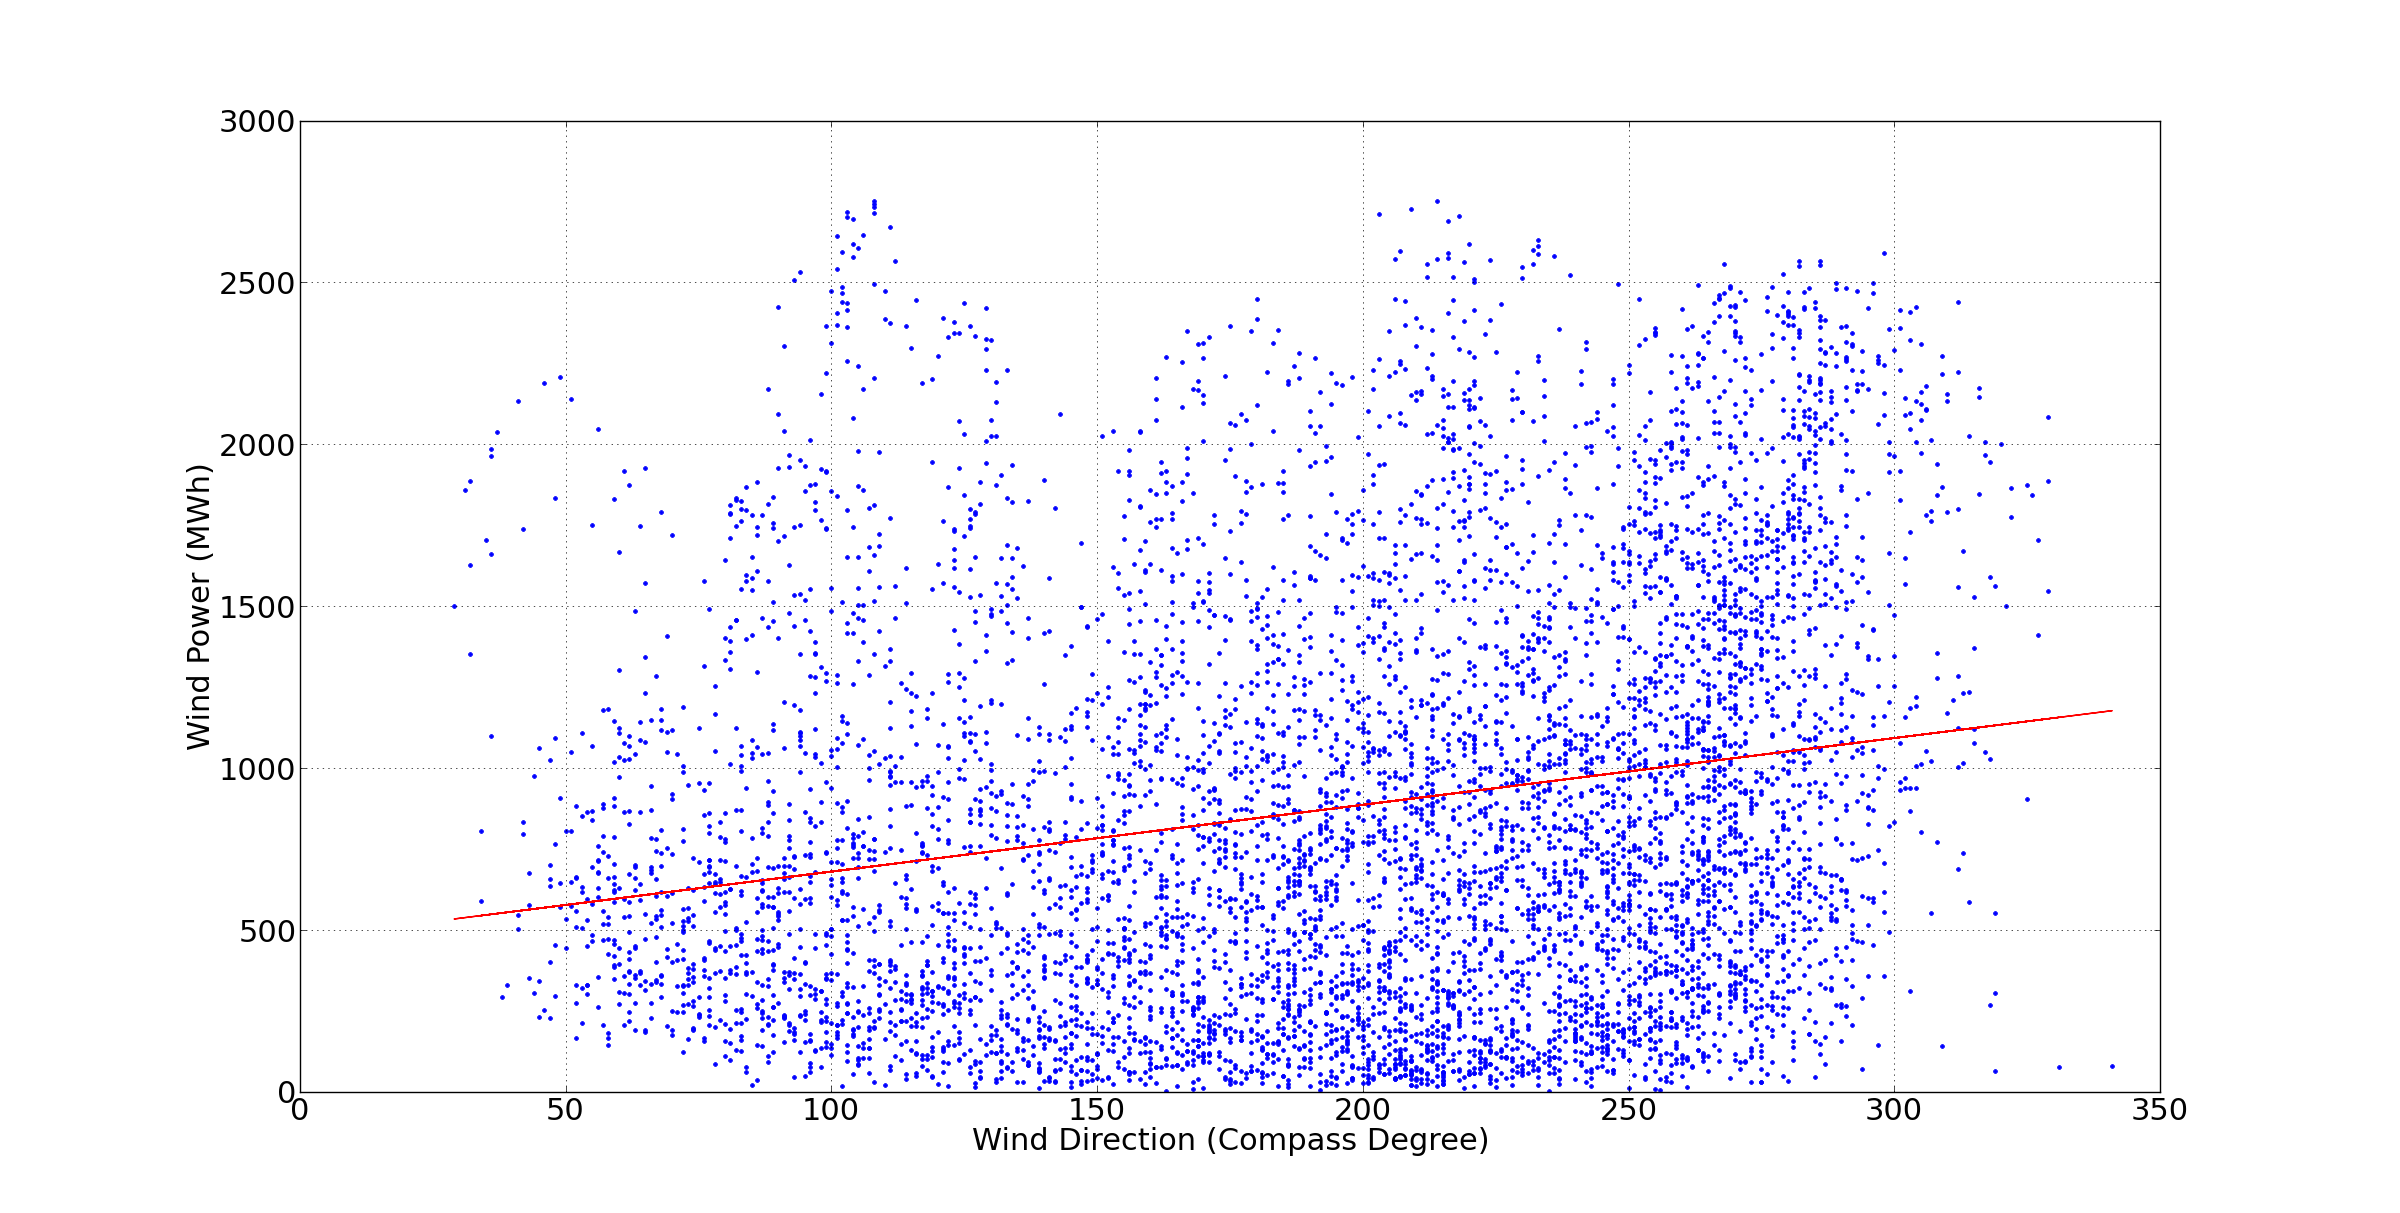
\includegraphics[width=0.99\linewidth,natwidth=898,natheight=587]{billeder/productionVsWindDirection.png}
\caption{Wind Direction vs. wind production in 2012}
\label{fig:windDirVsProd}
\end{figure}

\subsection{Consumption}
\label{sec:consumptionWindProduction}
It is expected that the wind power available on the energy market will be low at times with low consumption, e.g if no energy is needed the wind power can't be sold.  This relationship is shown in Figure~\ref{fig:consumptionVsWindProduction}. This also tells us that the wind production is connected to the market and cannot be deduced only from meteorological factors.

\begin{figure}[H]
\centering
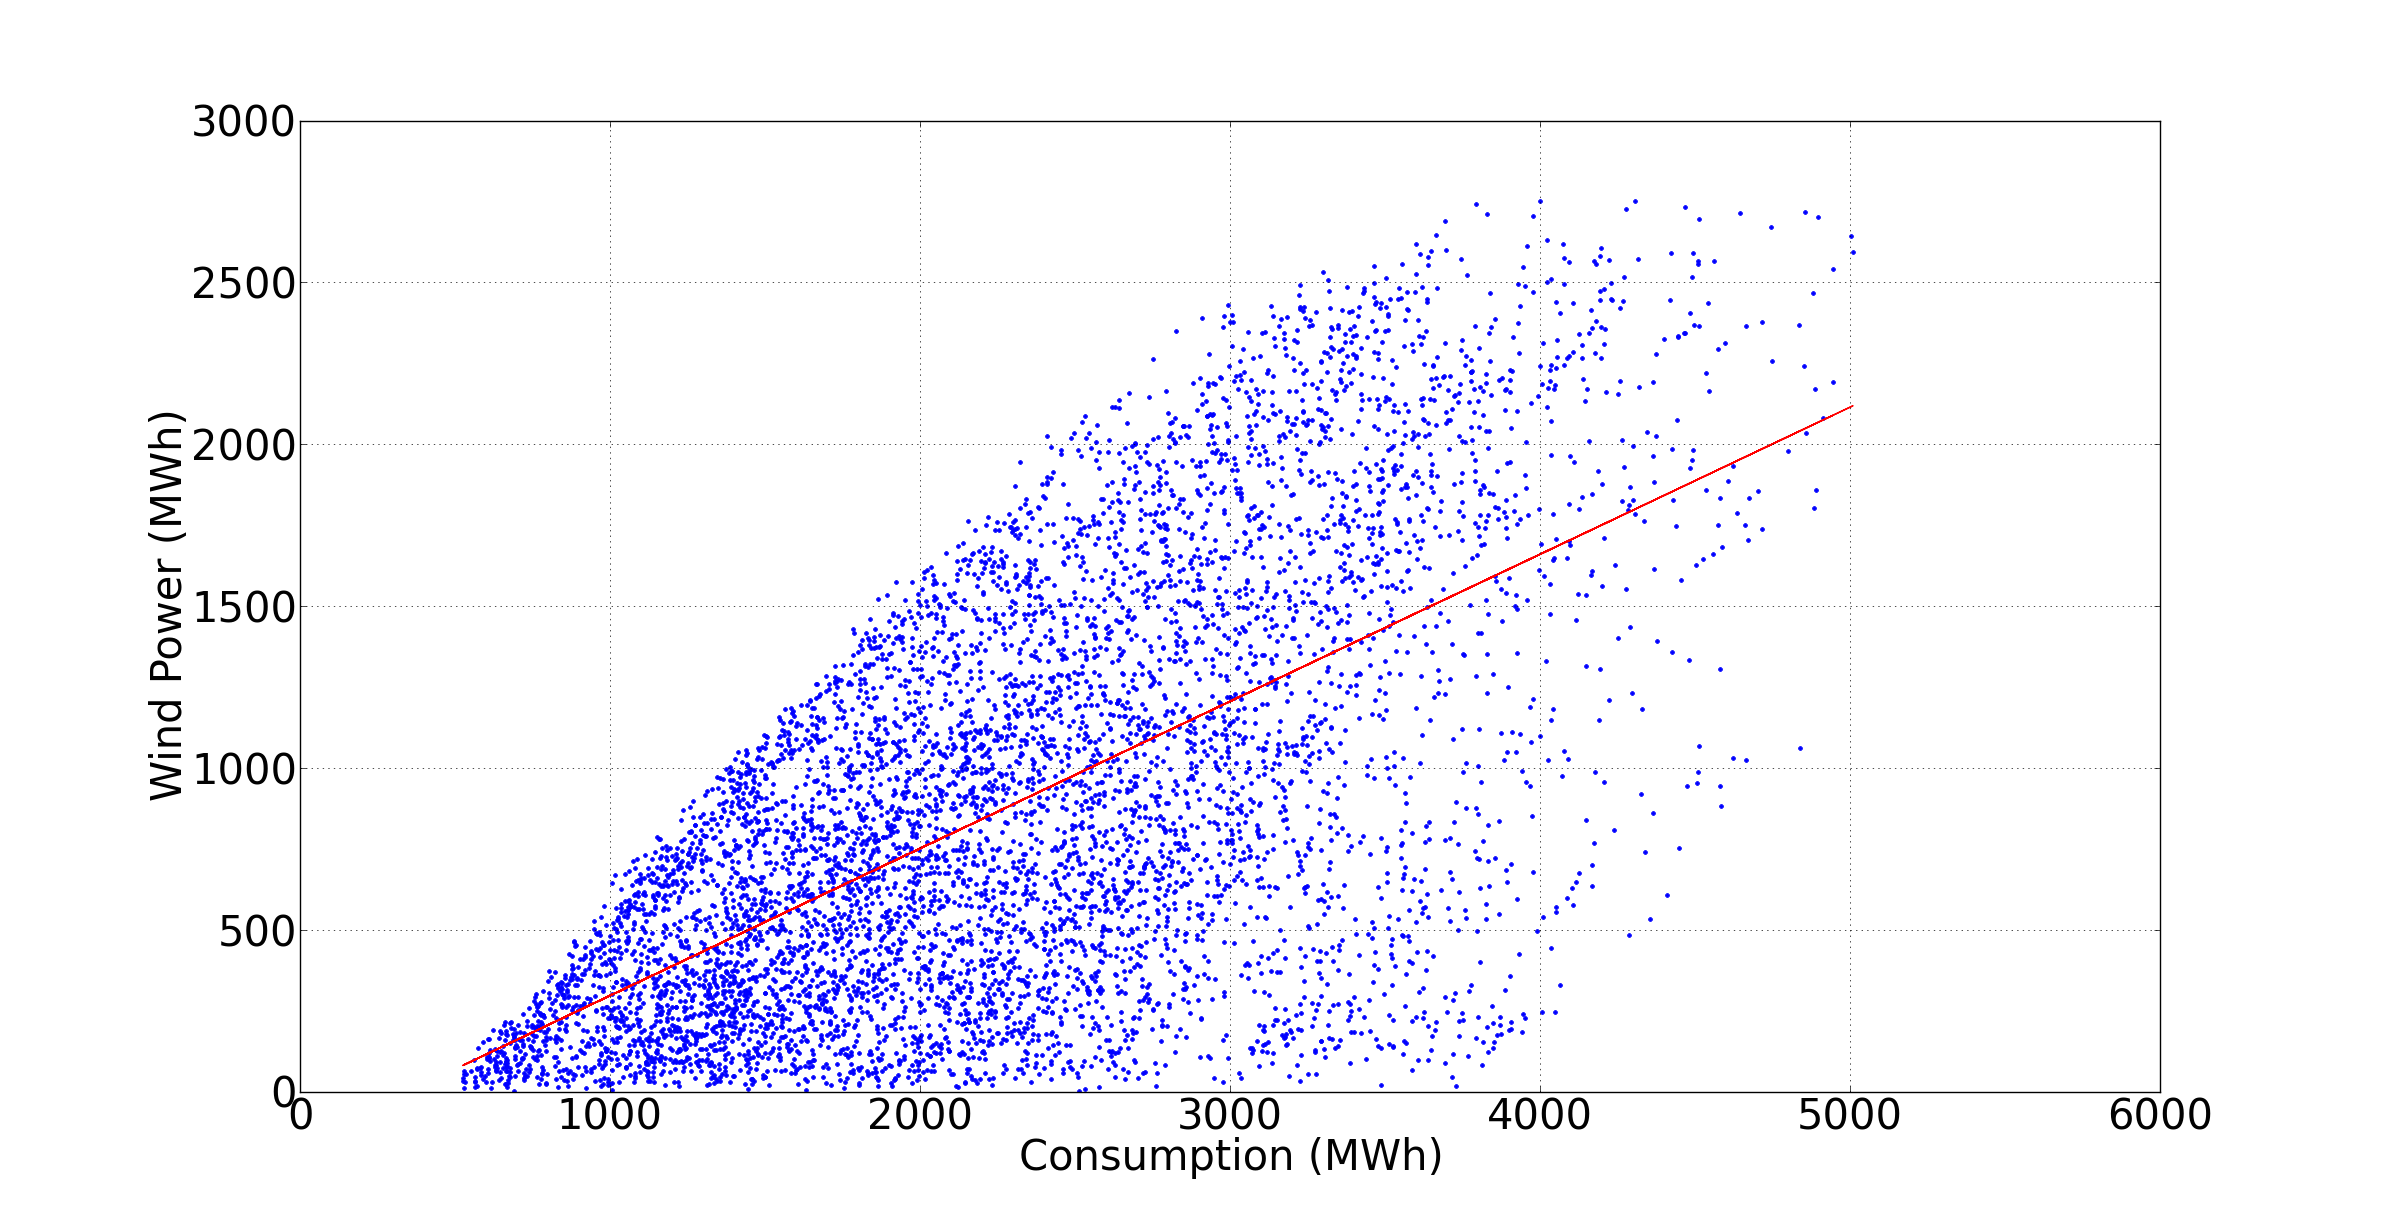
\includegraphics[width=0.99\linewidth,natwidth=898,natheight=587]{billeder/consumptionVsWindProduction.png}
\caption{Consumption vs. Wind Production in 2012}
\label{fig:consumptionVsWindProduction}
\end{figure}

It can be a disadvantage to use consumption as input since we will rely on predictions from nordpool spot - it is out of scope for this thesis to predict it in its own Neural Network. Following section~\ref{sec:ElectricityDemand} the demand is much controlled my the meteorological factors which can make it sufficient to include these as a substitute for the actual demand. The temperature impact on demand can be seen in Figure~\ref{fig:consump_temp_green}. We will compare the two approaches in experiments to come.

\begin{figure}[H]
\centering
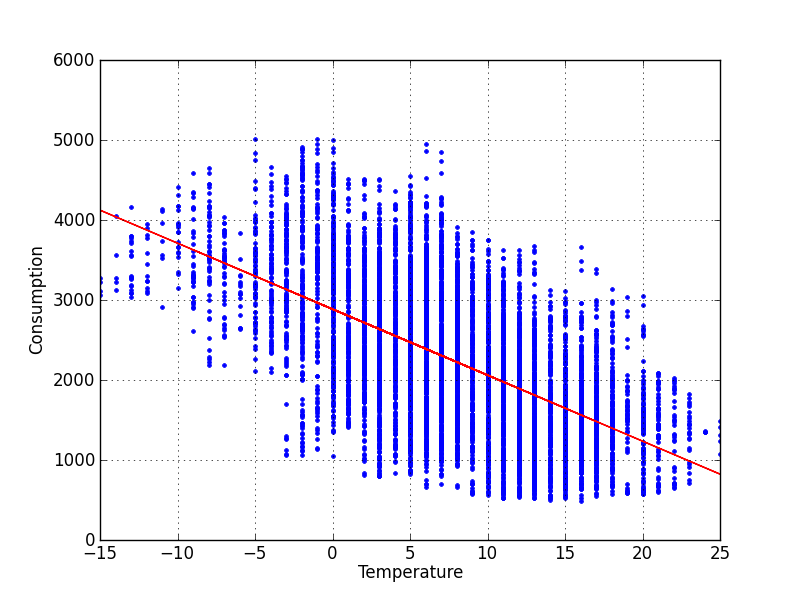
\includegraphics[width=0.8\textwidth ,natwidth=410,natheight=237]{billeder/energy_price_plots/consump_temp.png}
\caption{Demand and temperature plot.}
\label{fig:consump_temp_green}
\end{figure}

\subsubsection{Time of day}
\label{sec:greenTOD}
The dataset consists of all hours of the years included. Based on this the network is going to forecast multiple hours ahead and it therefore necessary to establish if any correlation between the time of day and the wind production exist. The average wind production distribution for a calendar day can be seen in Figure~\ref{fig:hourly_wind_production}. The wind production is at its highest during the day from 8-20 and therefore it is needed to use the time of day as input parameters.  

\begin{figure}[H]
\centering
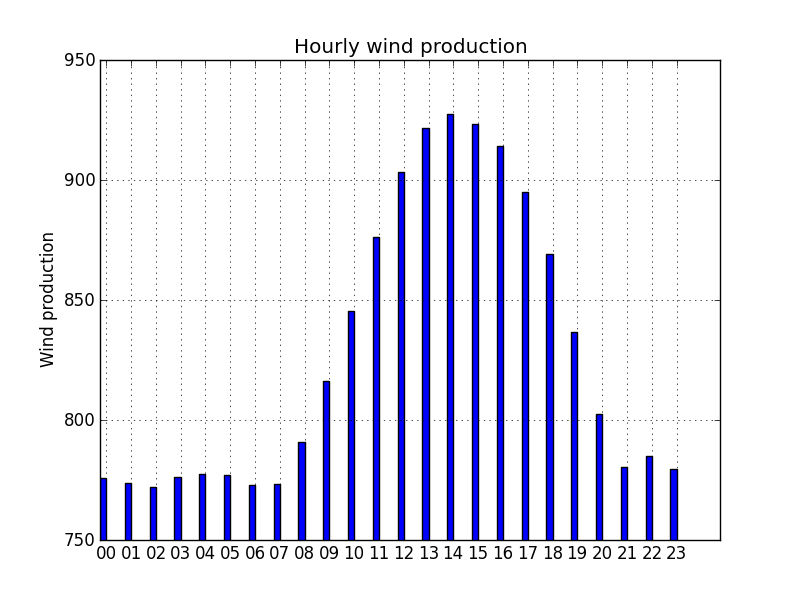
\includegraphics[width=0.99\linewidth,natwidth=898,natheight=587]{billeder/hourly_wind_production.png}
\caption{Time of day vs. Wind Production in 2012}
\label{fig:hourly_wind_production}
\end{figure}

\subsection{Seasonality}
\label{sec:windProdSeasonality}
The wind follows the seasons and the production follows the wind. The wind production should therefore vary according to the current season. This is validated by Figure~\ref{fig:windProductionMonths} and~\ref{fig:windProductionSeasons} where there is a significant distinction between summer and the other 3 seasonality.

\begin{figure}[H]
\centering
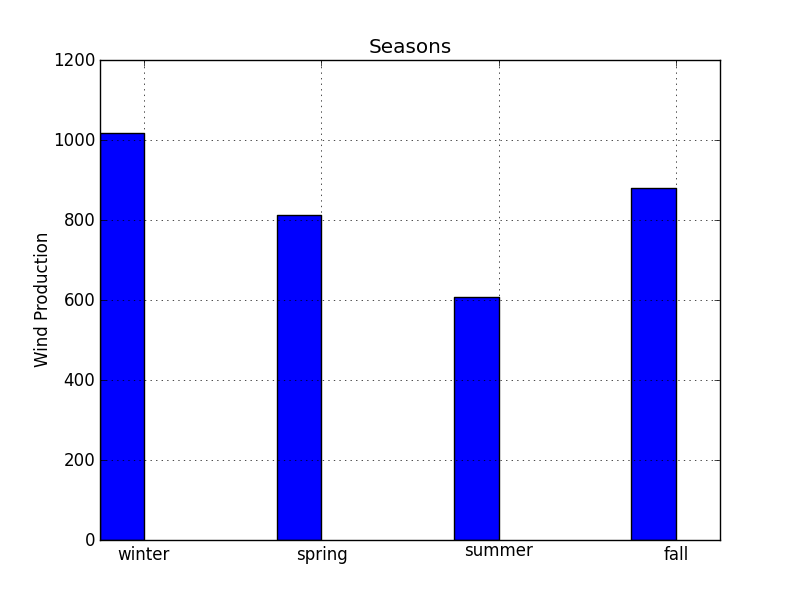
\includegraphics[width=0.99\linewidth,natwidth=898,natheight=587]{billeder/Seasons/windProdctionSeasons.png}
\caption{Wind production in relation to the four seasons in 2012}
\label{fig:windProductionSeasons}
\end{figure}

\begin{figure}[H]
\centering
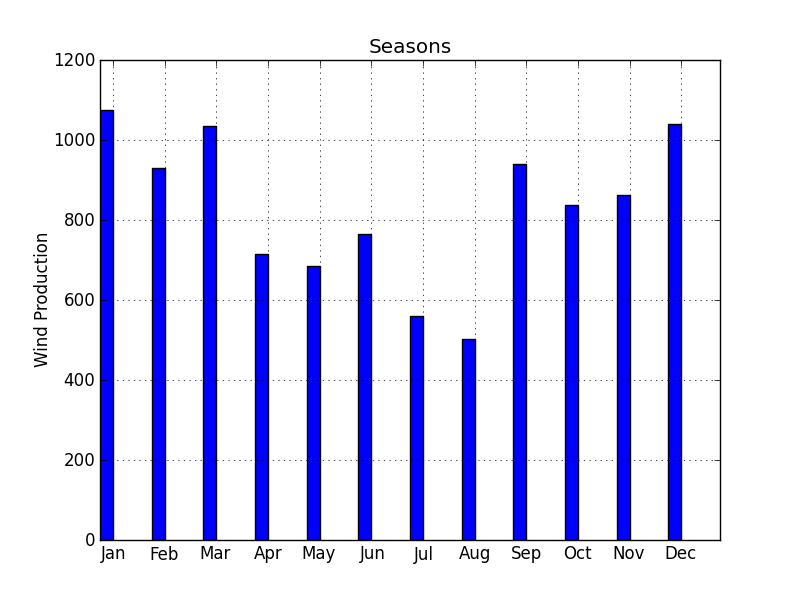
\includegraphics[width=0.99\linewidth,natwidth=898,natheight=587]{billeder/Seasons/windProductionMonths.png}
\caption{Wind production in relation to months in 2012}
\label{fig:windProductionMonths}
\end{figure}

\subsection{Wind Production Development}
\label{sec:windProductionDev}
The above analysis shows the wind production development to be much dependent on wind speed and air density together with the general trend on the market. 

The high volatility in the wind production is very clear when considering the development curve in Figure~\ref{fig:windHourDevelopment400Hours}. This is not a problem if the correlation between the input parameters result in a low number of output possibilities because the generalization of the ANN then would be enough. This is not the case for our input parameters for wind productions and an example of such can be seen in Figure ~\ref{fig:inputParameterDistribution} where outputs for similar inputs are shown --- the input limits can be seen in Table~\ref{table:similarHoursLimitsWindProd}. The generalization would lean towards 898-1048 but if the last wind production was 1198 and the tendency rising then the prediction would be better off guessing above or around 1198. This can be further supported by Figure~\ref{fig:windHourDevelopment400Hours} which illustrates the tendency of the production curve and the need to consider the immediate past because of its significance for the movements to come. Identifying these tendencies in every hour could possibly help the network to predict the wind production more accurately. The network already captures the trend of the entire training set but the more input parameters adding extra information about the individual hours the more accuracy could possibly be obtained. The point here is to give extra input information about the hours and the concept is discussed in more detail in Section~\ref{sec:usingStatisticalInput}. The simplest way to include information about the past is to include the production from past hours and let the network itself calculate the impact of former productions --- Figure~\ref{fig:windProductionVsLastWindProduction} shows the relationship between the current production and the last known production. The Pearson constant is here 0,99. Figure~\ref{fig:windHourDevelopment400Hours} shows that the production does not differ much from one hour to the next so by including the last known hour, the prediction could more accurately tell where it should place itself within the interval \todo{appendix that shit}. The statistics could then further strengthen this by analysing how if we should move or down and how much.

\begin{figure}[H]
\centering
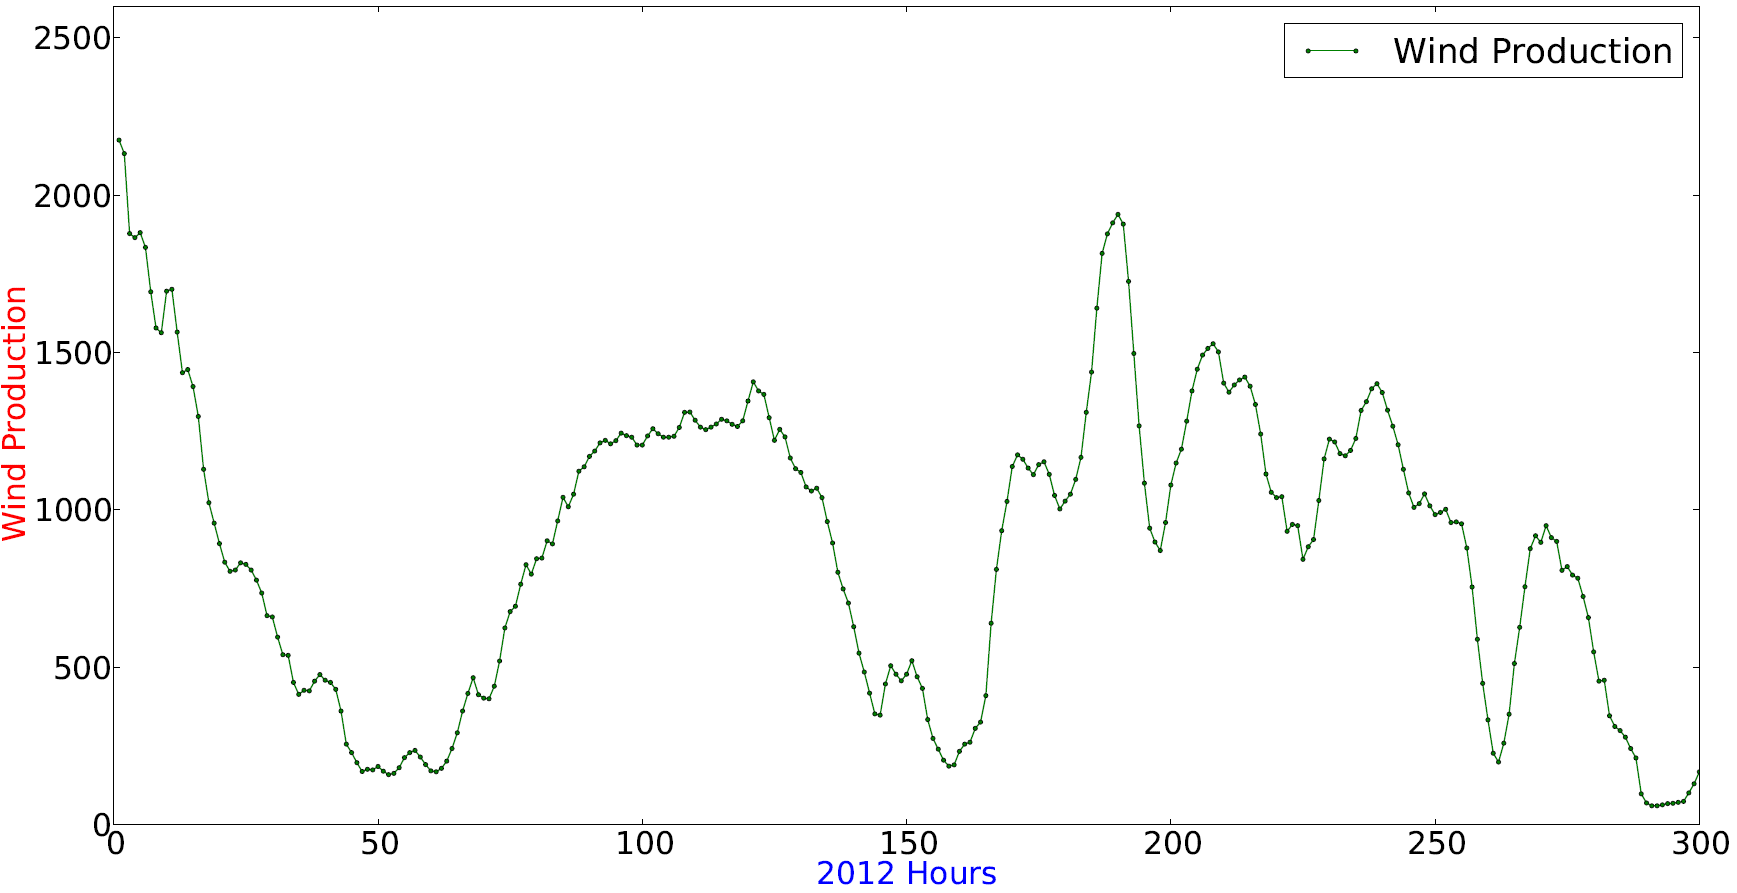
\includegraphics[width=0.99\linewidth,natwidth=898,natheight=587]{billeder/productionTendency400Hours.png}
\caption{Wind production development for 400 hours in 2011}
\label{fig:windHourDevelopment400Hours}
\end{figure}

\begin{figure}[H]
\centering
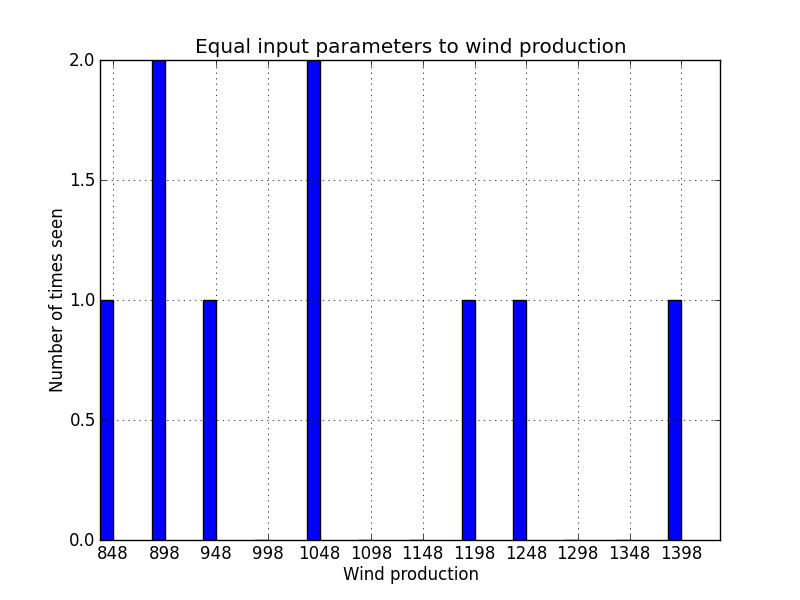
\includegraphics[width=0.99\linewidth,natwidth=898,natheight=587]{billeder/Equal_wind.png}
\caption{Same input parameter to wind production output distribution}
\label{fig:inputParameterDistribution}
\end{figure}

\begin{table}[H]
\centering  % used for centering table
\begin{tabular}{c c c c} % centered columns (3 columns)
 & \#1 Windspeed & \#2 Temperature (Celsius) & \#3 Demand \\ [0.5ex] % inserts table 
%heading
\hline                  % inserts single horizontal line
High margin: & 16.5 & 3.3 & 2359.5  \\
Low margin: & 13.5 & 2.7 & 1930.5 \\ [1ex] % [1ex] adds vertical space
\hline %inserts single line
\end{tabular}
\caption{This is the high and low margins used for the the similar input to output distribution.} % title of Table
\label{table:similarHoursLimitsWindProd} % is used to refer this table in the text
\end{table}

Figure~\ref{fig:windHourDevelopment400Hours} does not show any need for trimming when predicting wind production over an entire year. The curve of wind production does not contain any cases that are unpredictable, e.g productions that suddenly drops without any intermediary steps. 

Different percentage of trims for an entire year can be seen in Figure~\ref{fig:windProductionTrimming}. The cutting of productions will result in the network being able to predict those specific values when they are seen during the year to predict. This is valid if the values are out of the ordinary or unpredictable which is not the case for the wind power production. The curve contains only one irregular drop in the hours between 1200-1300 where the production suddenly drops to zero. The rest of the curve does not make sudden jumps and it follows intermediary steps or trends. When predicting wind power production for an entire year trimming should be omitted. It will be discussed later if it in the hands of a trader could make sense to trim data based on expertise, e.g. the trader knows the production from the last hour to 300 and due to the knowledge about trend choose to trim away the training dataset above 1800 because experience tells that it most likely does not reach this height. Trimming will only make sense if the predictions achieve better accuracy on the same values as the prediction values without trimming.

\begin{figure}[H]
\centering
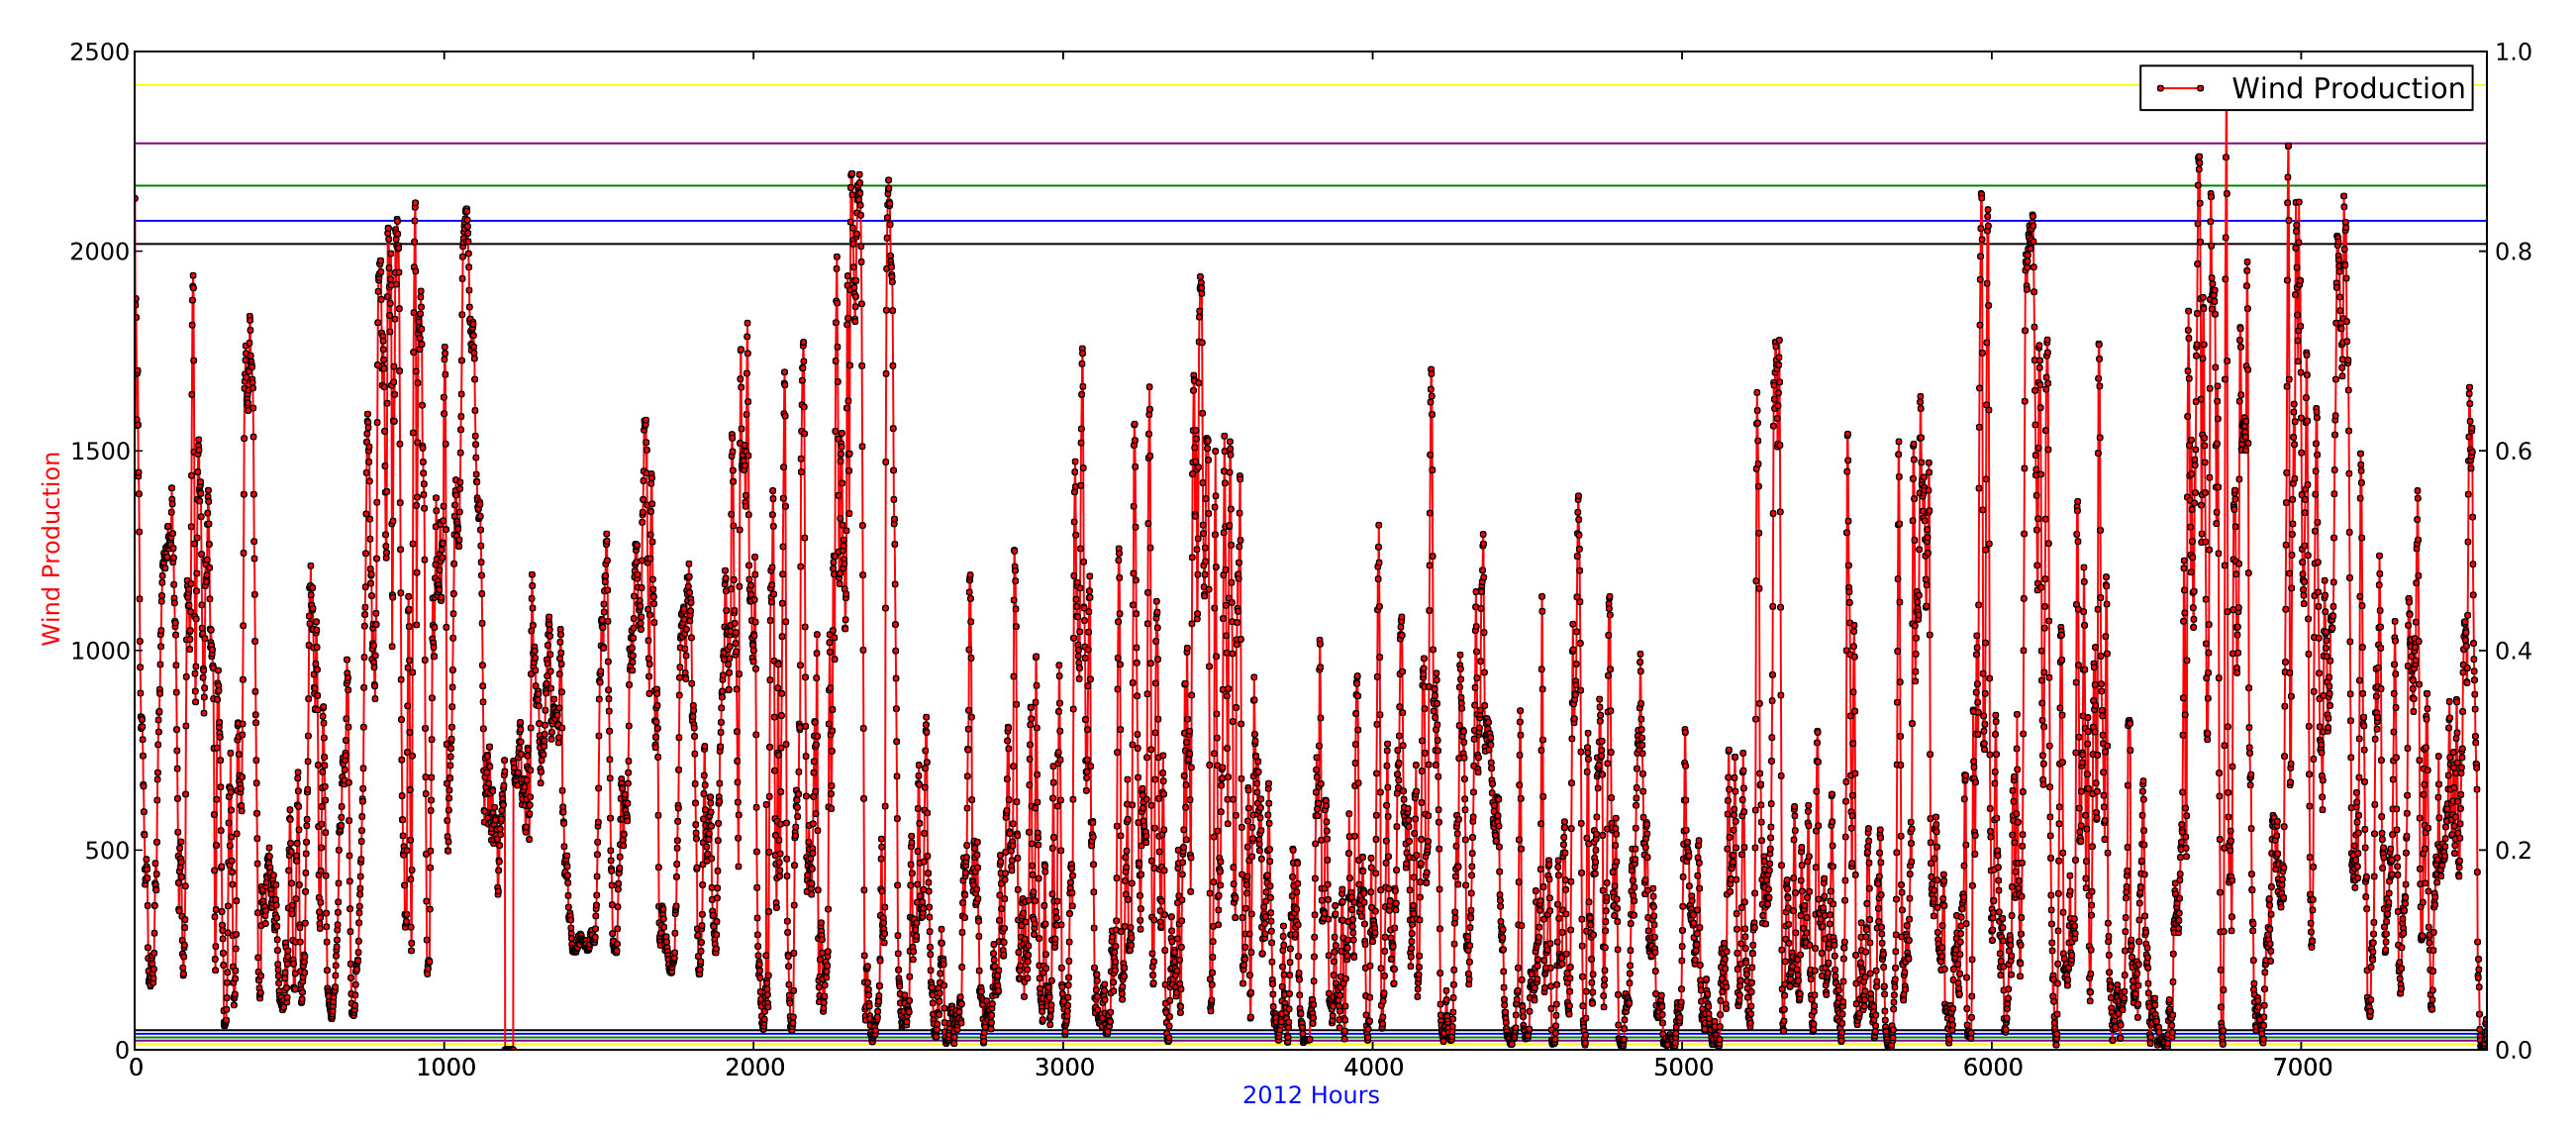
\includegraphics[width=0.99\linewidth,natwidth=898,natheight=587]{billeder/windProductionTrimming.jpg}
\caption{Wind power production trimming}
\label{fig:windProductionTrimming}
\end{figure}

\begin{figure}[H]
\centering
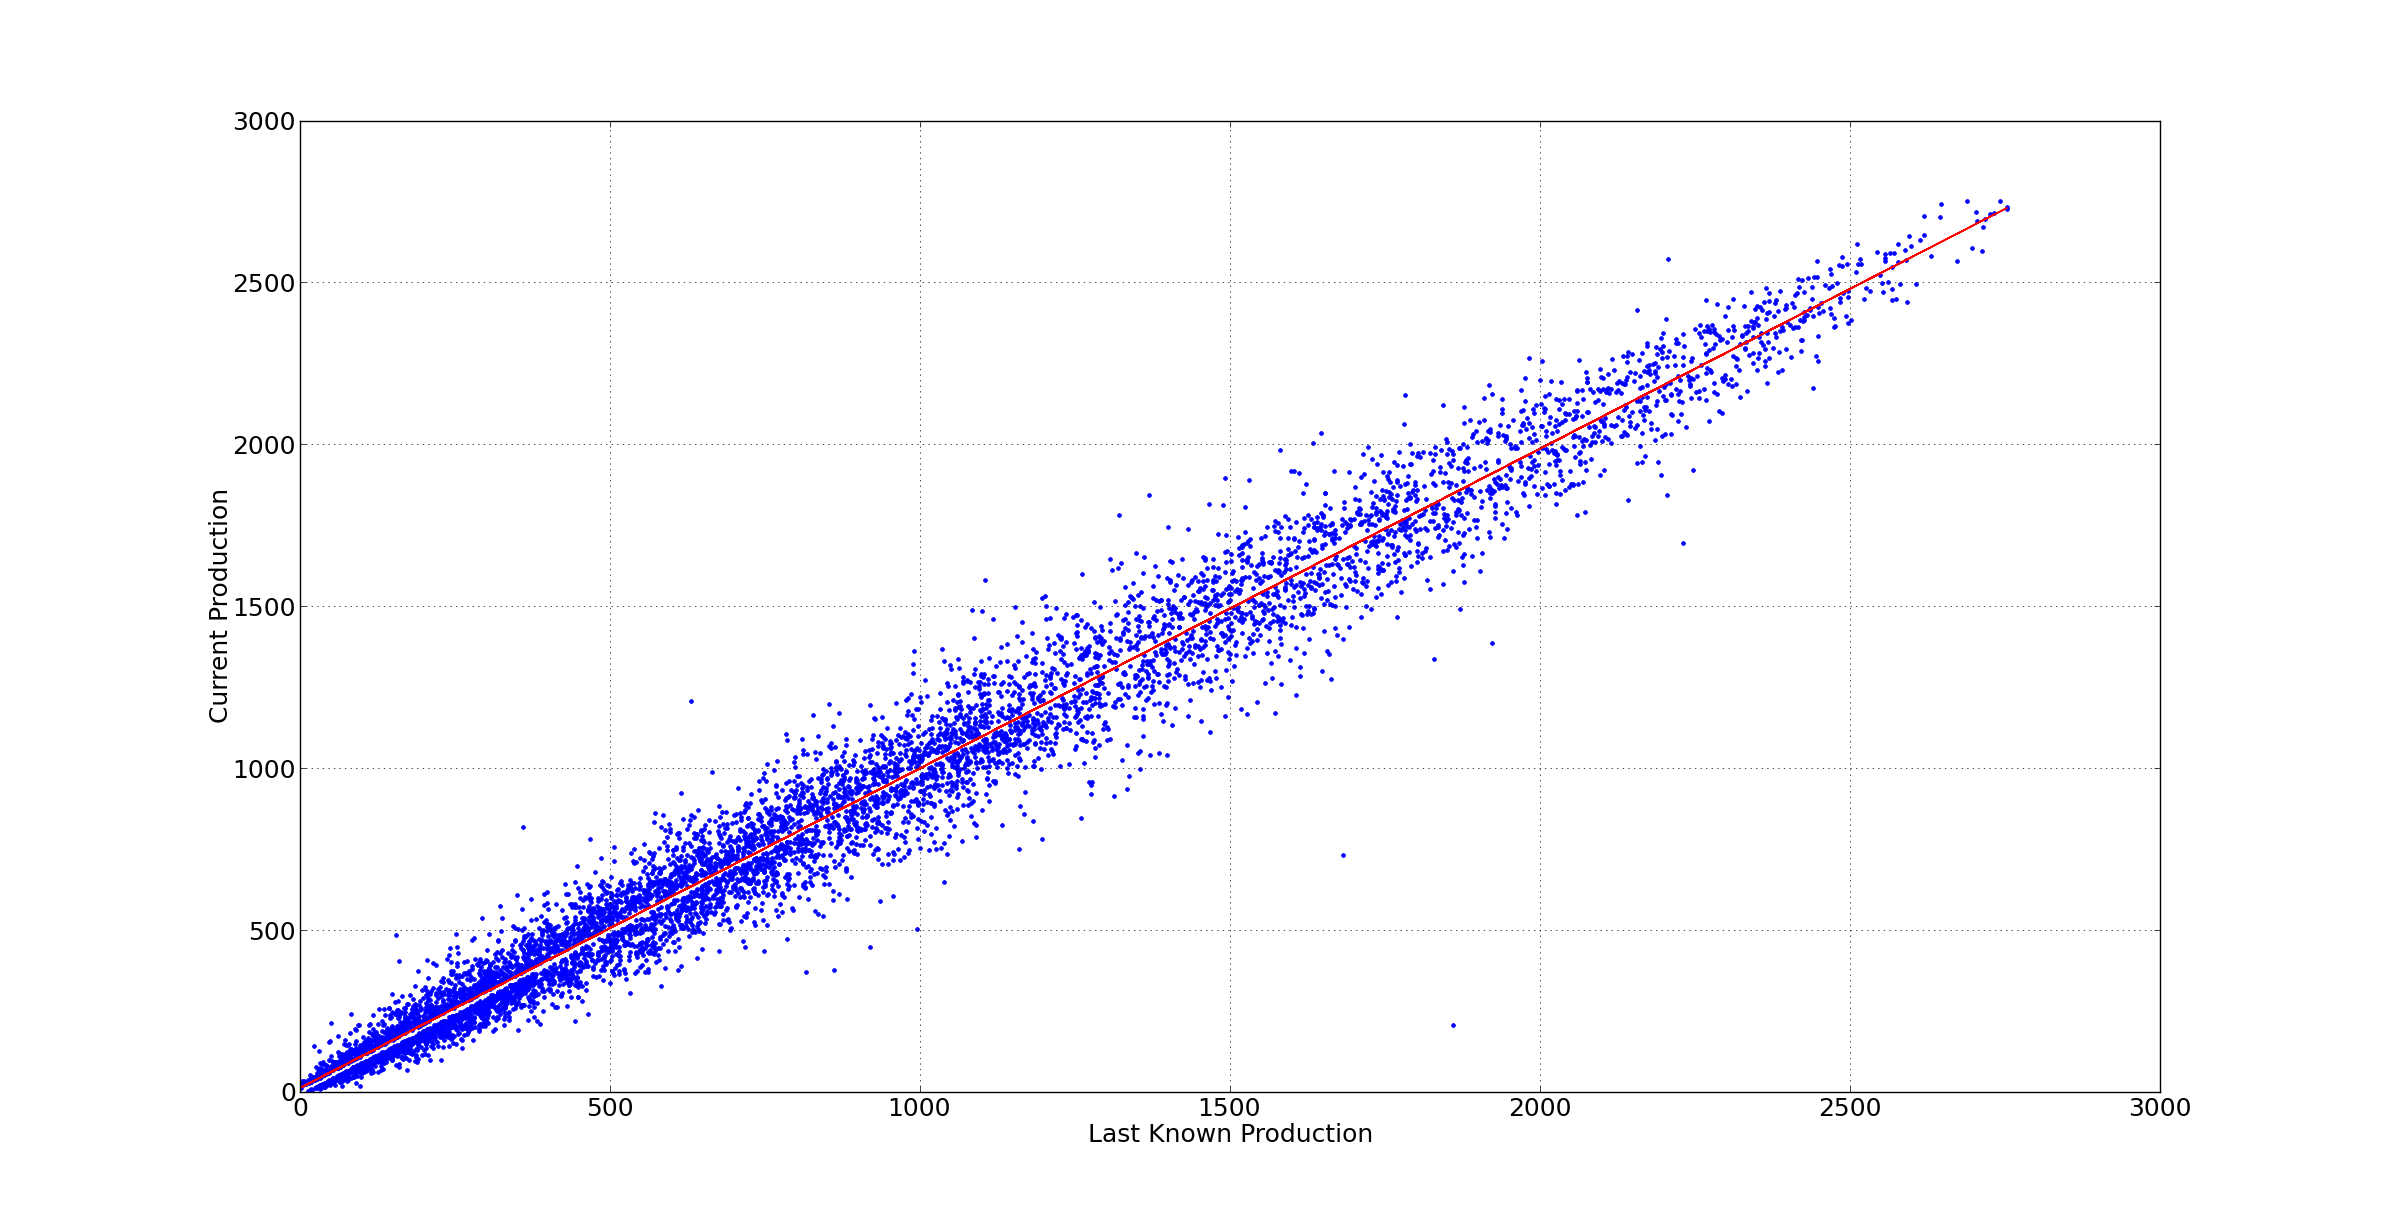
\includegraphics[width=0.99\linewidth,natwidth=898,natheight=587]{billeder/windProductionVsLastWindProduction.png}
\caption{Wind power production vs. last known wind power production}
\label{fig:windProductionVsLastWindProduction}
\end{figure}

\subsection{Conclusion}
The above analysis has clarified to what extend the different parameters effect the wind production. Not surprisingly wind speed has the greatest influence and wind production followed same trends, but also consumption has shown to have a good co-relation with the production which tells us about a link to the electricity market. The wind production vary from hour to hour which makes the time of day a significant factor. The wind production is decreased significantly during winter so the season will also need to be included in test. The analysis of the wind production development showed the need for including past productions for better knowing the movements to come.
The air density is according to its formula proportional to wind production and it showed a co-relation of 0,28 in average. The current wind direction and wind production showed a co-relation but further validation needs to be carried out in experiments.